\documentclass{beamer}
\setbeamertemplate{navigation symbols}{}

\usetheme{Madrid}
\usecolortheme{beaver}

% packages
\usepackage{graphicx}
\usepackage{enumitem}

% metadata
\title{Fault-Tolerant Quadcopter}
\author{Cooper, Vaughn, Mayank}
\date{\today}

\begin{document}

% title slide
{\setbeamertemplate{footline}{}
\begin{frame}
\begin{center}
{\Large\textbf{Fault-Tolerant Quadcopter}}\\
\vspace{\baselineskip}
ECE 453 Project Proposal (Fall 2018)\\
University of Wisconsin-Madison\\
\vspace{\baselineskip}
{\large\textit{Vaughn Kottler, Mayank Katwal, Cooper Green}}
\end{center}
\end{frame}
}

% state of the art (cheap toys)
\begin{frame}
\frametitle{State of the Art (Cheap Toys)}
\begin{center}
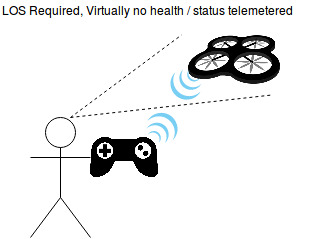
\includegraphics[width=3.5in]{../src/im/crude}

Price Range: \$25 - \$50
\end{center}
\end{frame}

% state of the art (fpv)
\begin{frame}
\frametitle{State of the Art (Enthusiast FPV)}
\begin{center}
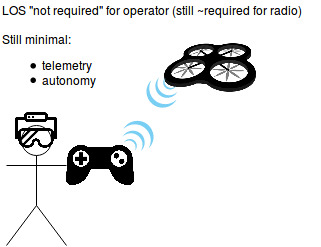
\includegraphics[width=3.5in]{../src/im/fpv}

Price Range: \$100+
\end{center}
\end{frame}

% state of the art (industry)
\begin{frame}
\frametitle{State of the Art (Industry)}
\begin{center}
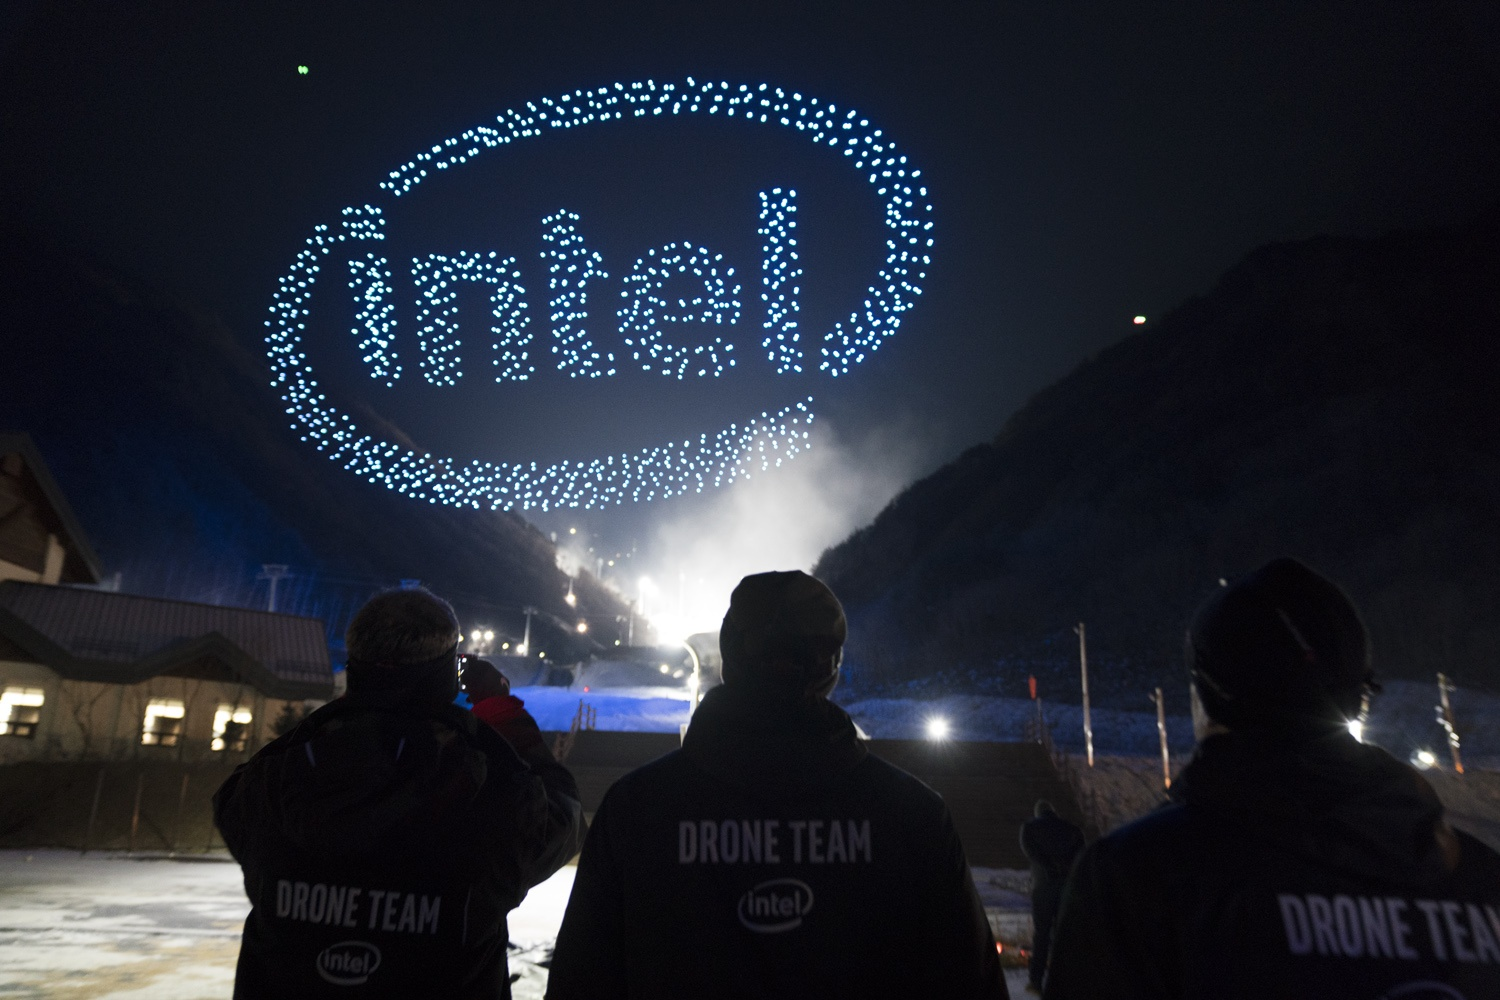
\includegraphics[width=4in]{../src/im/autonomous2}

Light Show at the Olympics
\end{center}
\end{frame}

% state of the art (industry)
\begin{frame}
\frametitle{State of the Art (Industry)}
\begin{center}
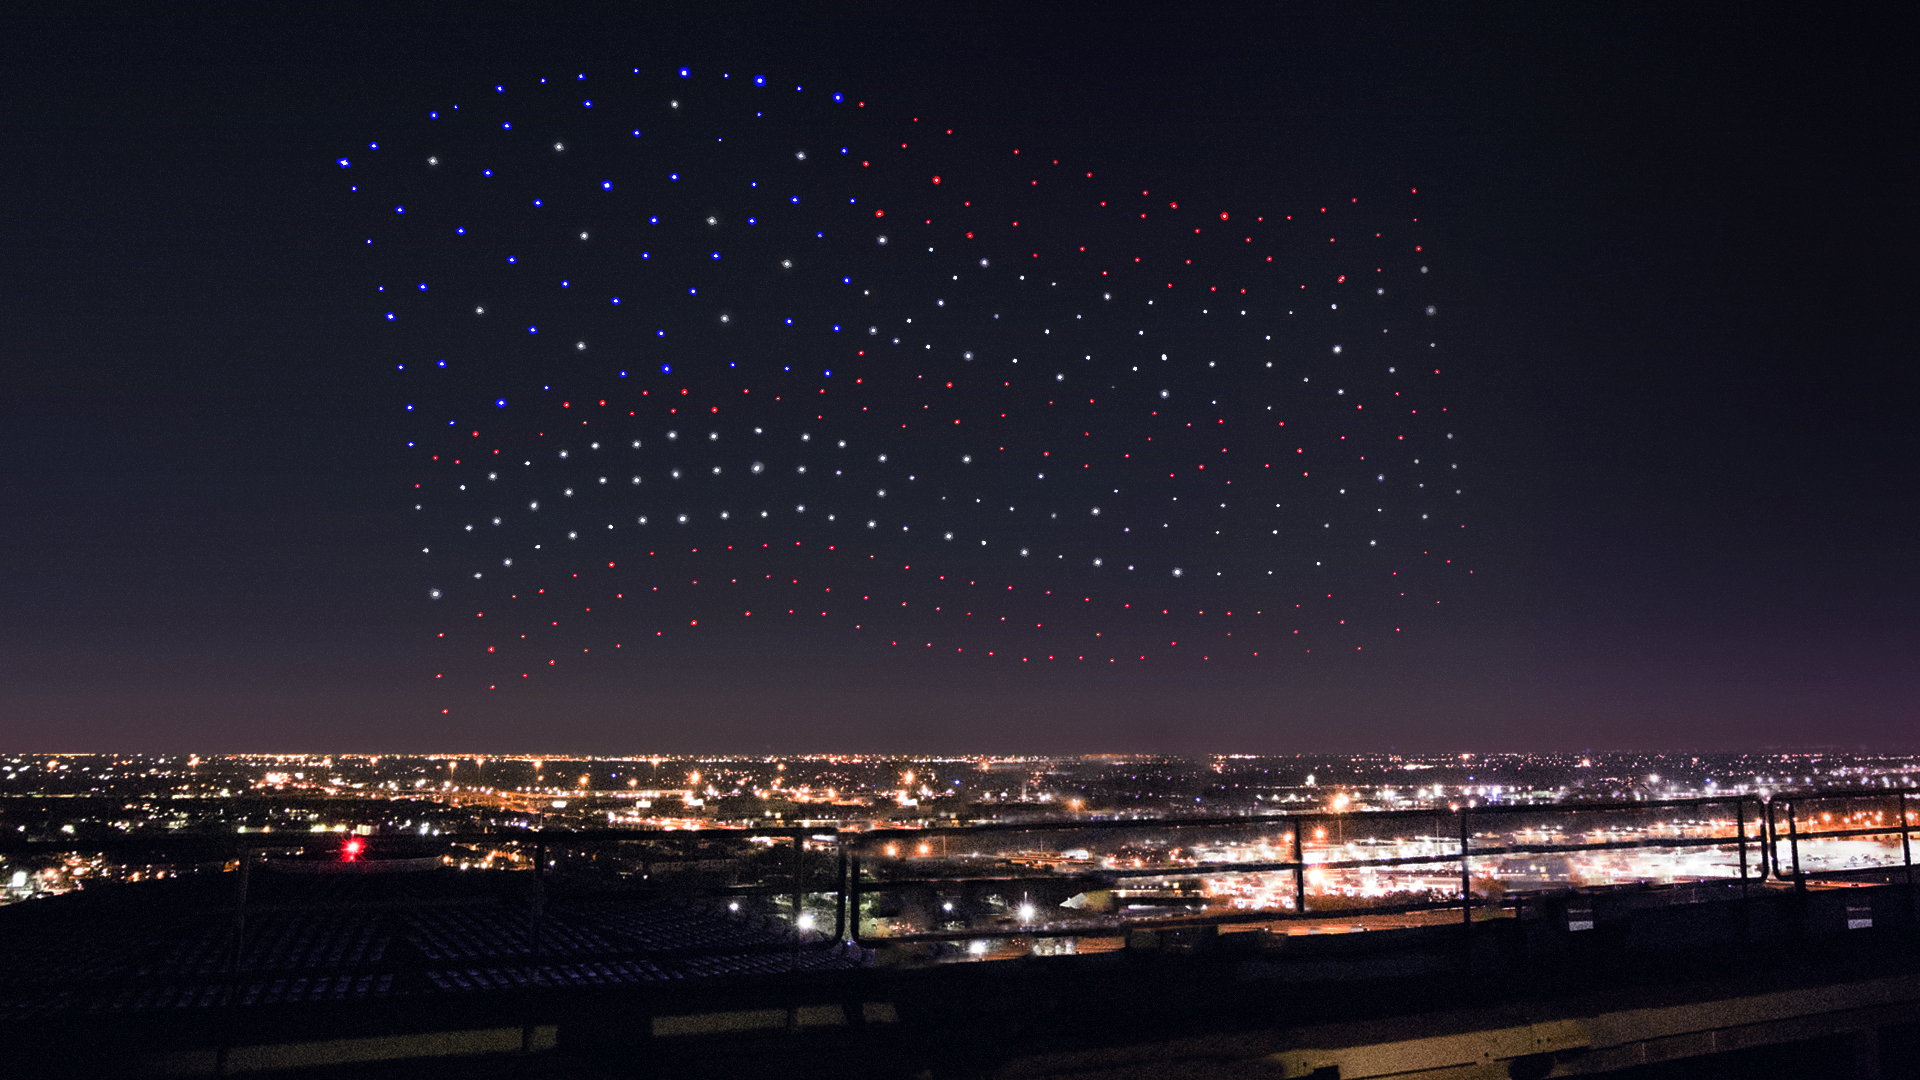
\includegraphics[width=4in]{../src/im/autonomous3}

Super Bowl LI Halftime Show
\end{center}
\end{frame}

% state of the art (industry)
\begin{frame}
\frametitle{State of the Art (Industry)}
\begin{center}
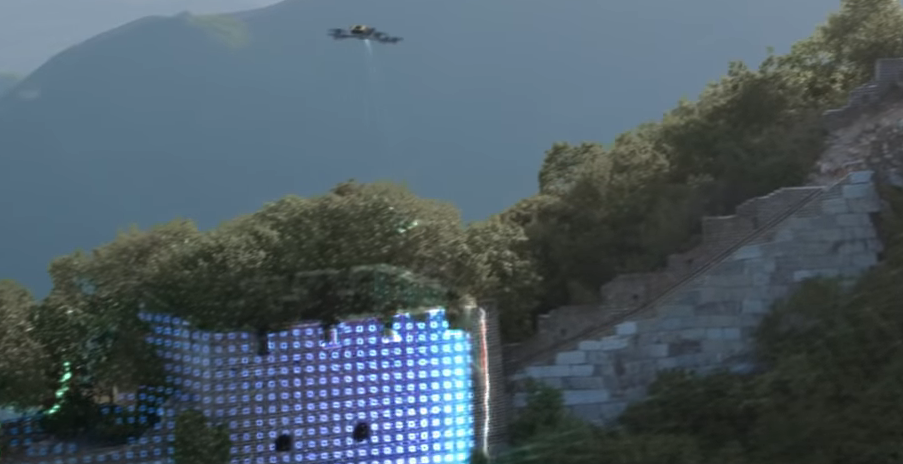
\includegraphics[width=4in]{../src/im/great_wall1}

Intel Surveys Great Wall of China
\end{center}
\end{frame}

% state of the art (industry)
\begin{frame}
\frametitle{State of the Art (Industry)}
\begin{center}
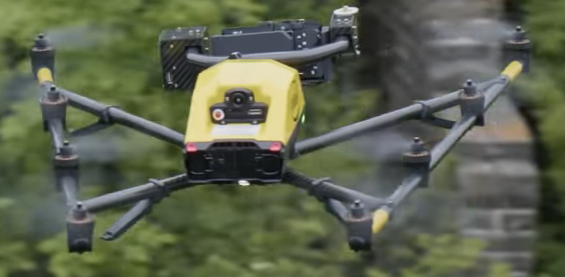
\includegraphics[width=2.5in]{../src/im/great_wall2}
\break
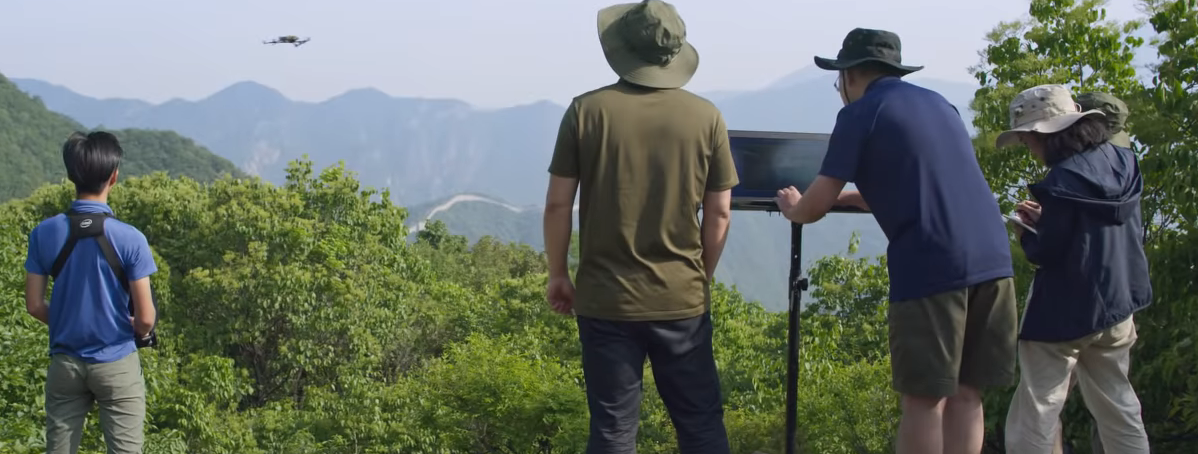
\includegraphics[width=3.5in]{../src/im/great_wall3}

Controlled via laptop
\end{center}
\end{frame}

% problem statement
\begin{frame}
\frametitle{Problem Statement - Motivation}
\Large
To gain relevant experience with aerospace problem spaces, it's necessary
to design, test and build a custom flying machine.
\break

\textbf{How hard are these problems?}
\end{frame}

% problem statement
\begin{frame}
\frametitle{Problem Statement - Relevance}
\Large
Seemingly no ``multi-vehicle fleet'' or autonomous-flight capable drone
technology is available to interact with in the consumer market.
\break

\textbf{We gap can we fill in this ecosystem?}
\end{frame}

% concept of approach
\begin{frame}
\frametitle{Concept of Operation}
\begin{center}
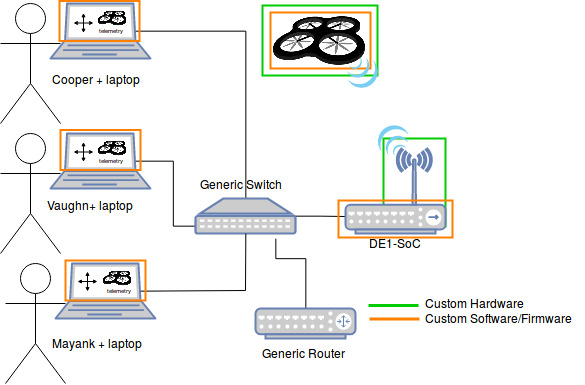
\includegraphics[width=4.5in]{../src/im/conops}
\end{center}
\end{frame}

% top-level block diagram
\begin{frame}
\frametitle{Overview}
\begin{center}
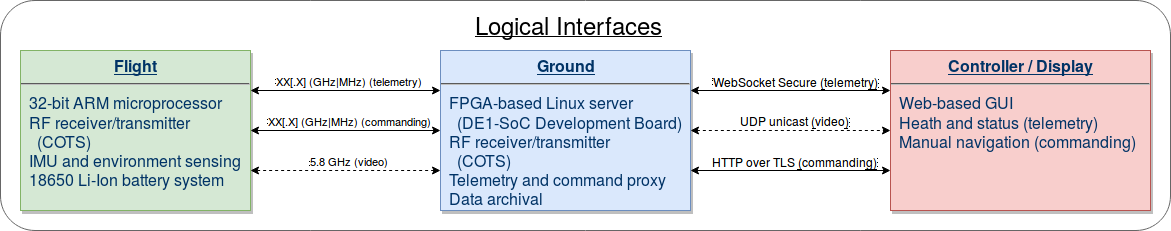
\includegraphics[width=\linewidth]{../src/im/top_level}
\end{center}
\vspace{\baselineskip}
\begin{description}[align=right,labelwidth=80pt,itemsep=10pt]
\item [Quadcopter] -- Battery-powered, four-motor flying machine
\item [Ground Station] -- Linux server managing the quadcopter's
	radio endpoint, hosts wired-network services (i.e.\ telemetry)
\item [Web-based UI] -- A modern dashboard for visualizing data
	and manually commanding the vehicle
\end{description}
\end{frame}

% features
\begin{frame}
\frametitle{Features}
\begin{description}[align=right,labelwidth=120pt,itemsep=10pt]
	\item [Single-Fault Tolerant] -- Land safely in the event of communication
		``heartbeat timeout''
	\item [Telemetry Archival] -- Implement long-term telemetry storage for
		post-flight data analysis
\end{description}
\end{frame}

% quadcopter
\begin{frame}
\frametitle{Quadcopter}
\begin{center}
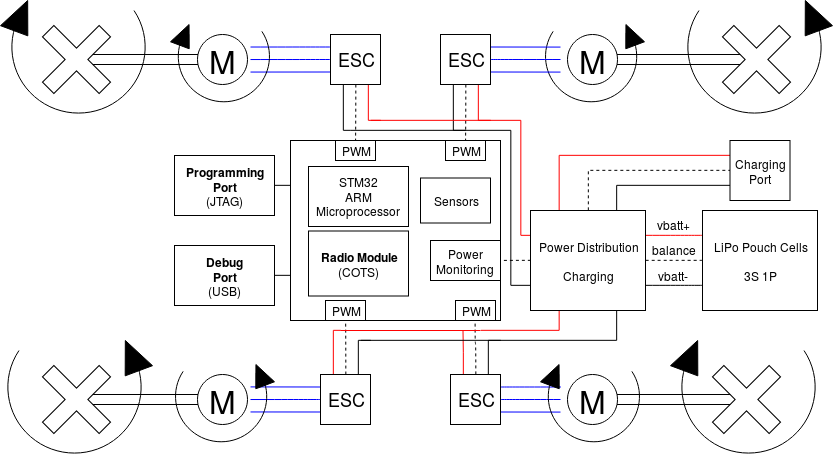
\includegraphics[width=\linewidth]{../src/im/quadcopter}
\end{center}
\end{frame}

% quadcopter components
\begin{frame}
\frametitle{Quadcopter Components}
\begin{center}
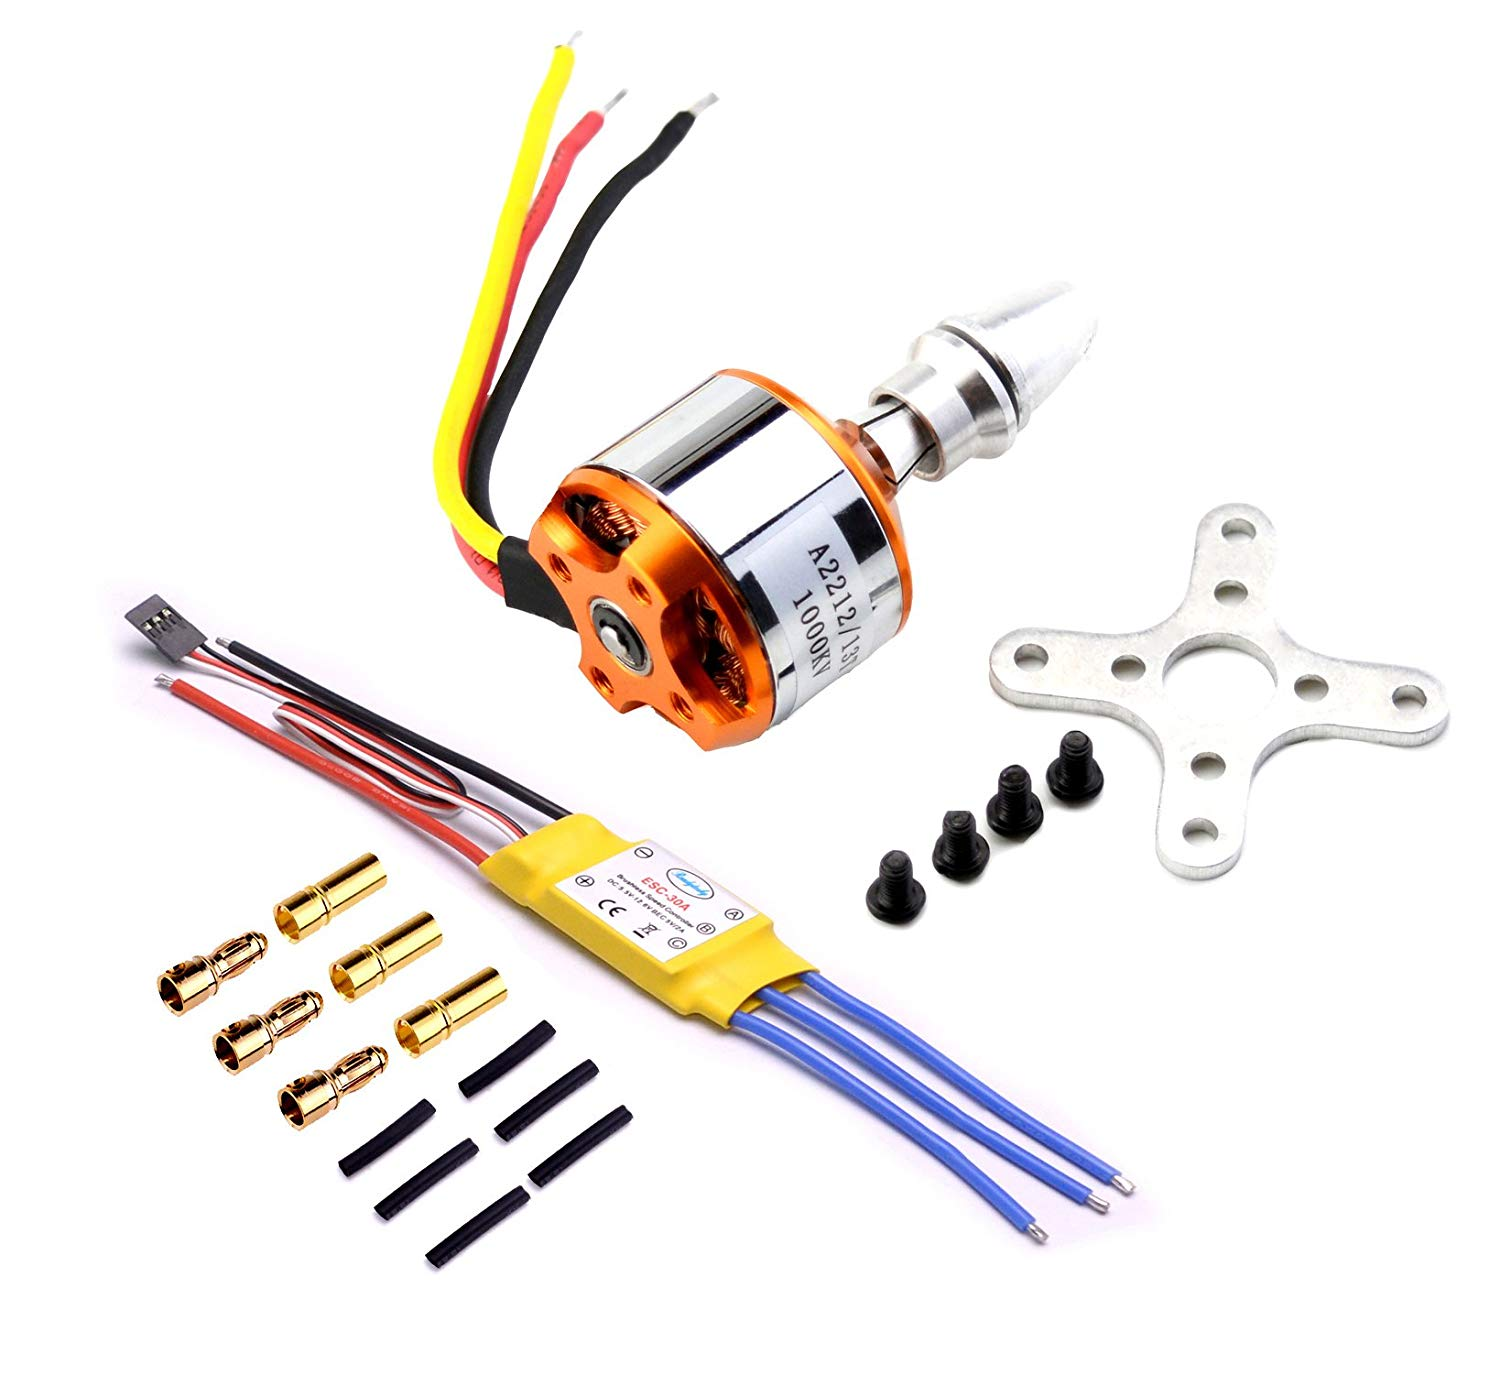
\includegraphics[width=1in]{../src/im/motor_esc}
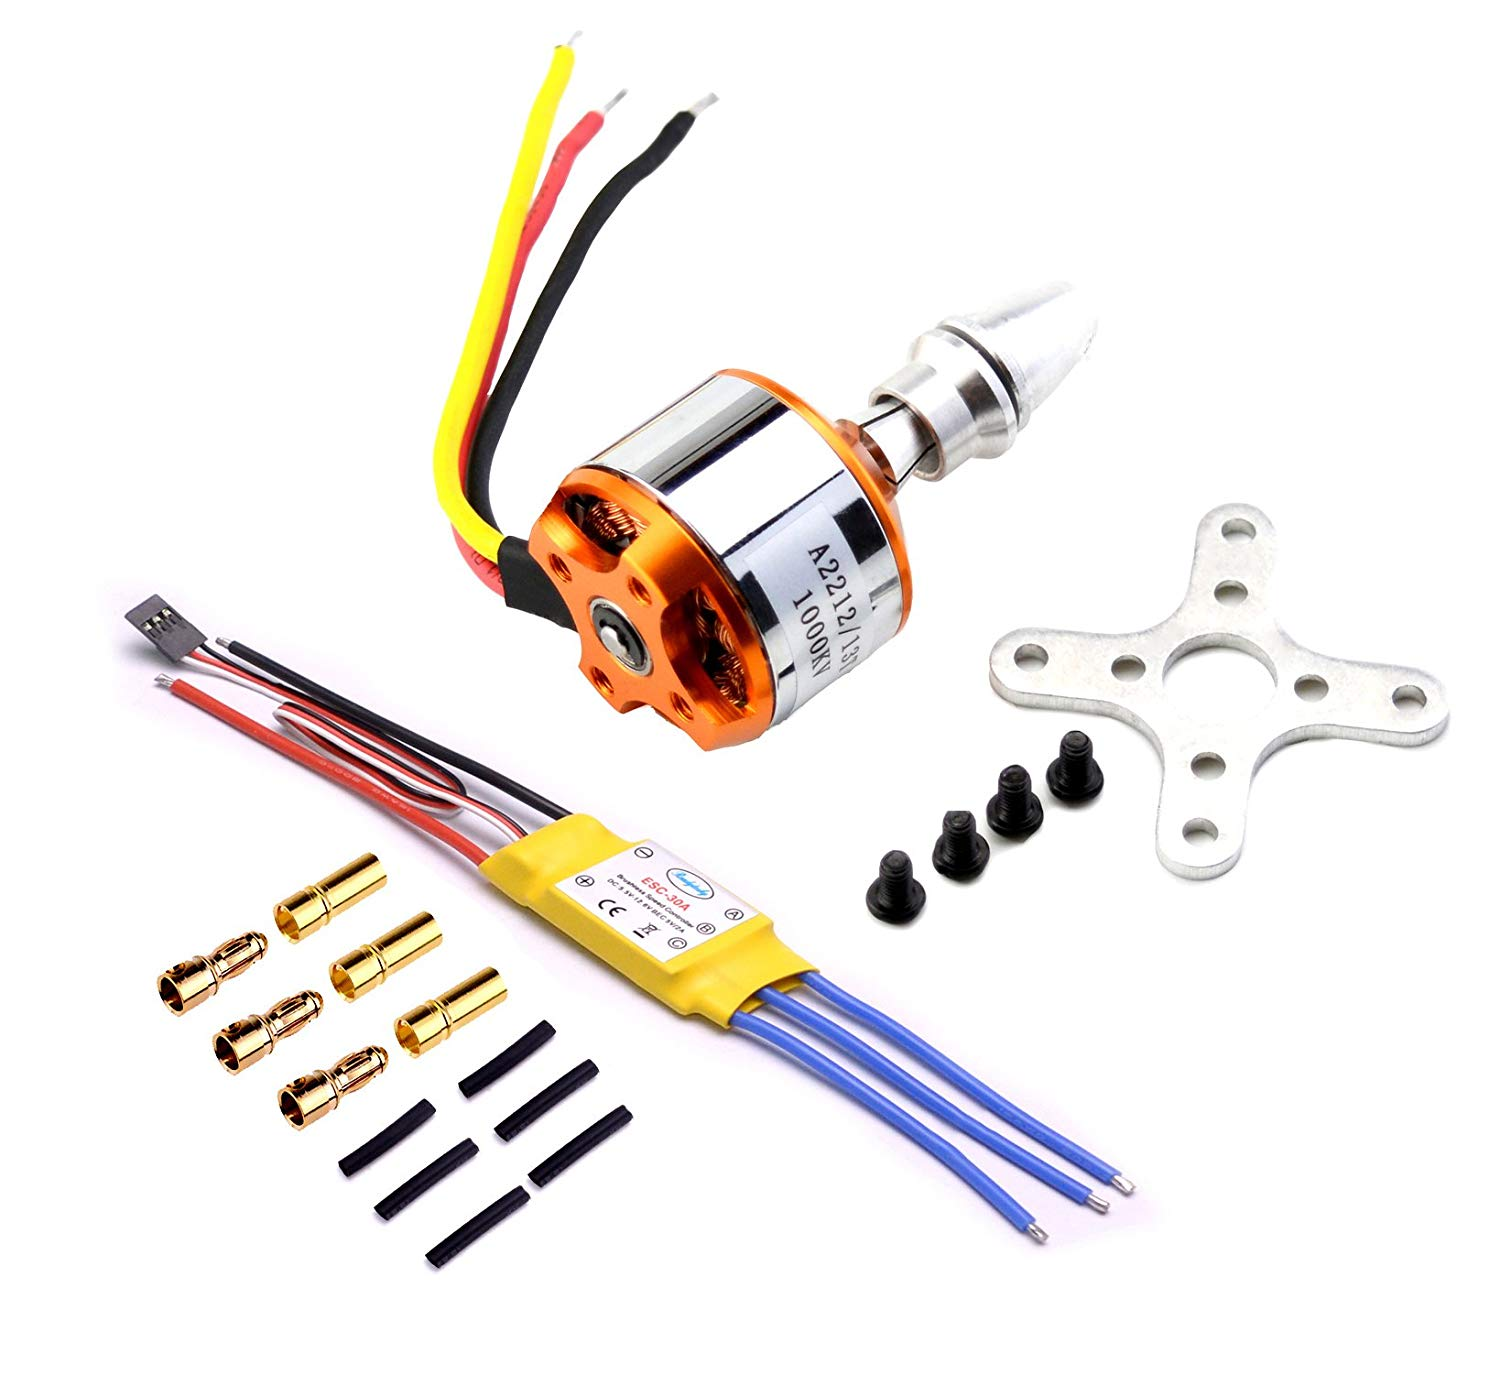
\includegraphics[width=1in]{../src/im/motor_esc}
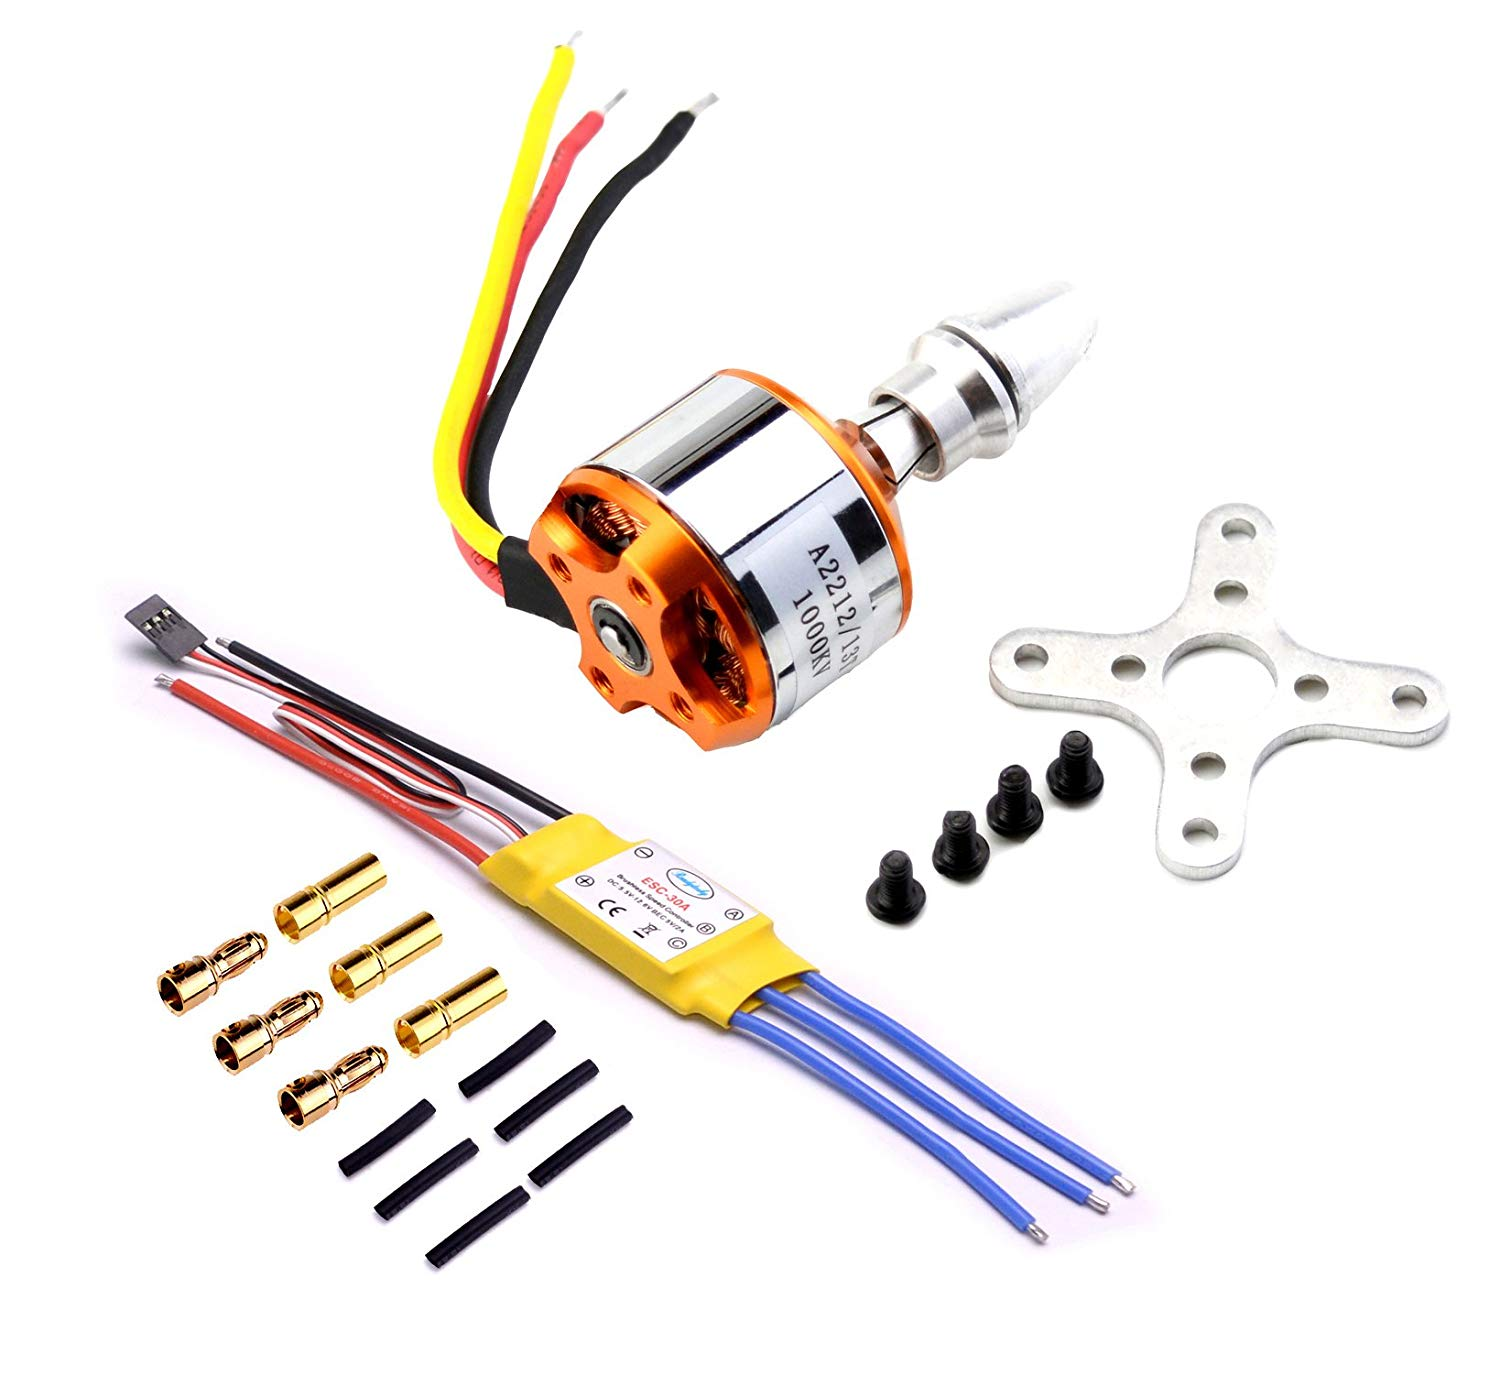
\includegraphics[width=1in]{../src/im/motor_esc}
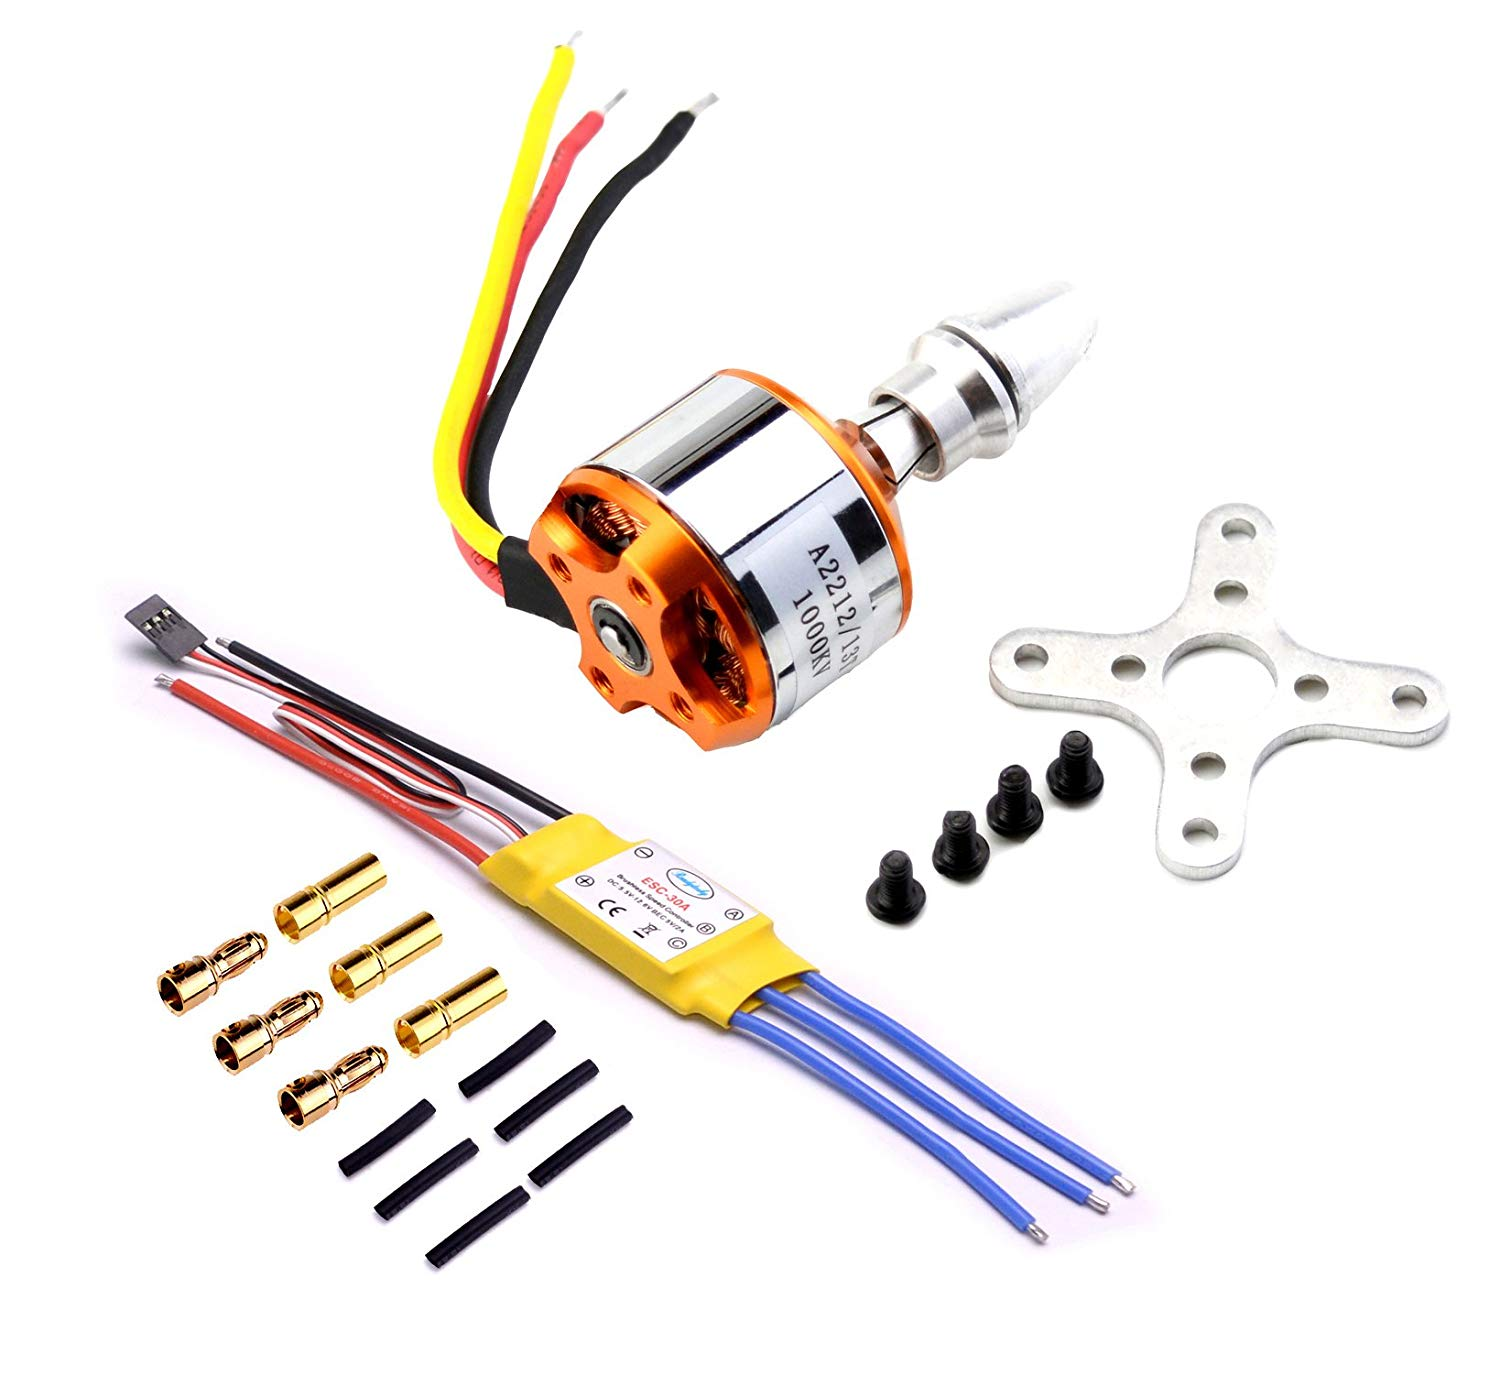
\includegraphics[width=1in]{../src/im/motor_esc}
\break
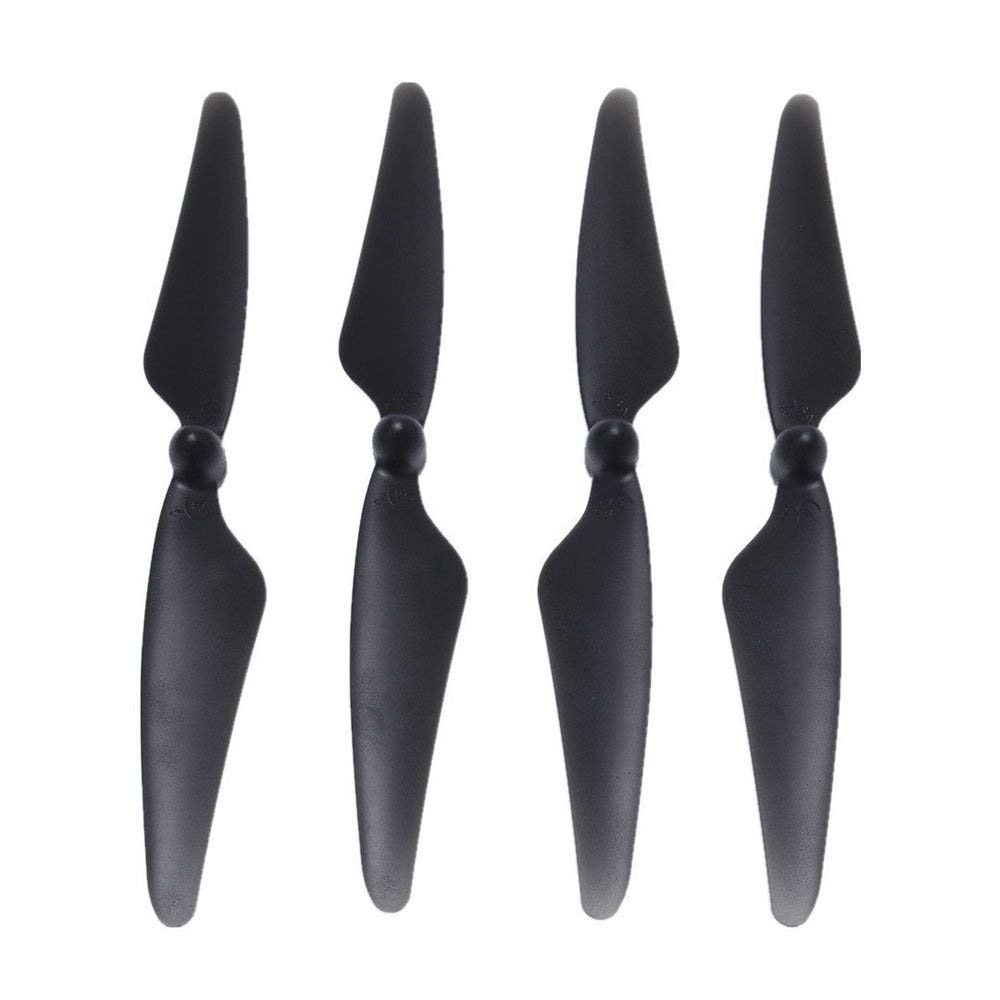
\includegraphics[width=1in]{../src/im/propeller}
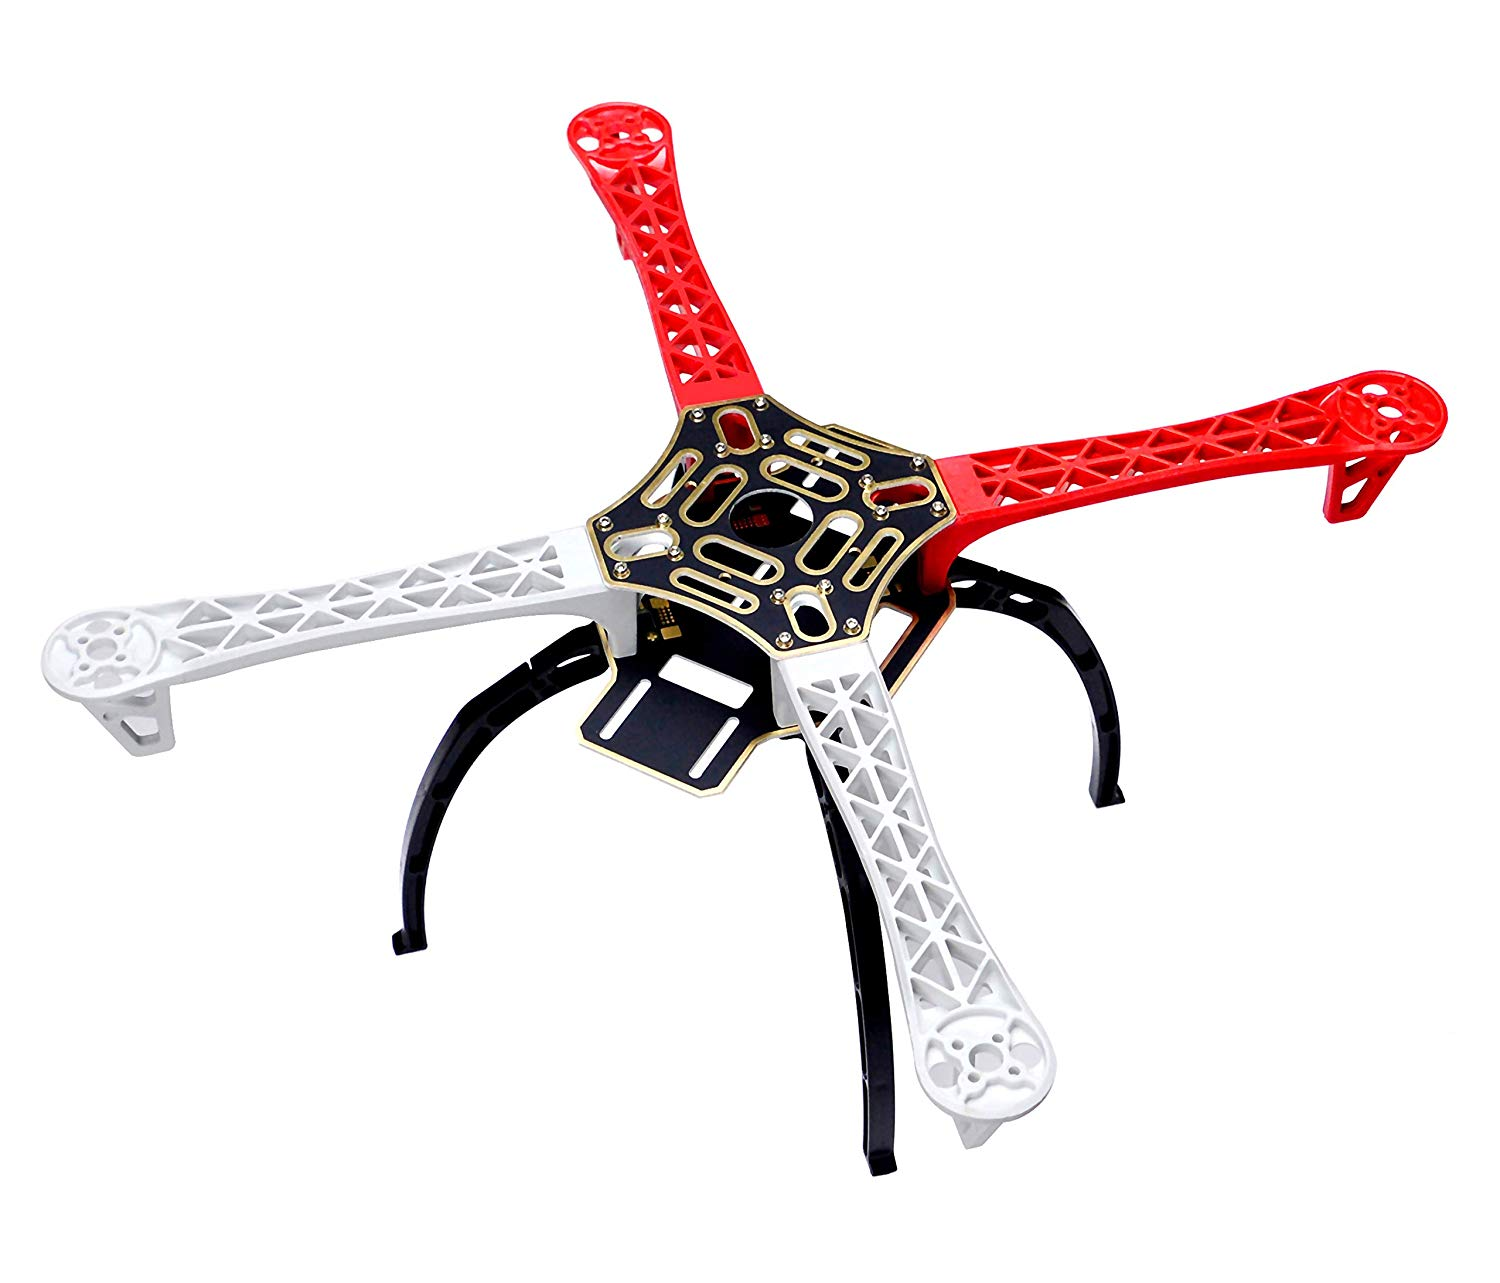
\includegraphics[width=1in]{../src/im/chassis}
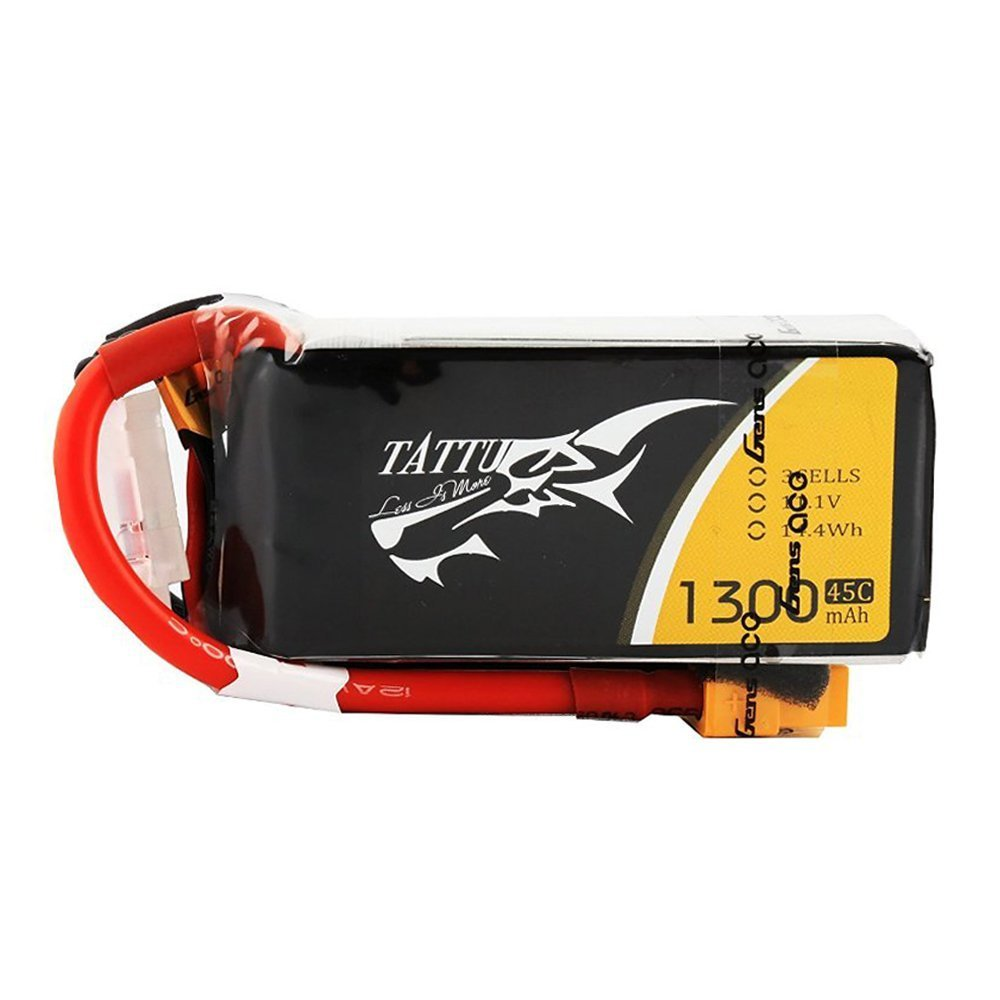
\includegraphics[width=1in]{../src/im/battery}
\break
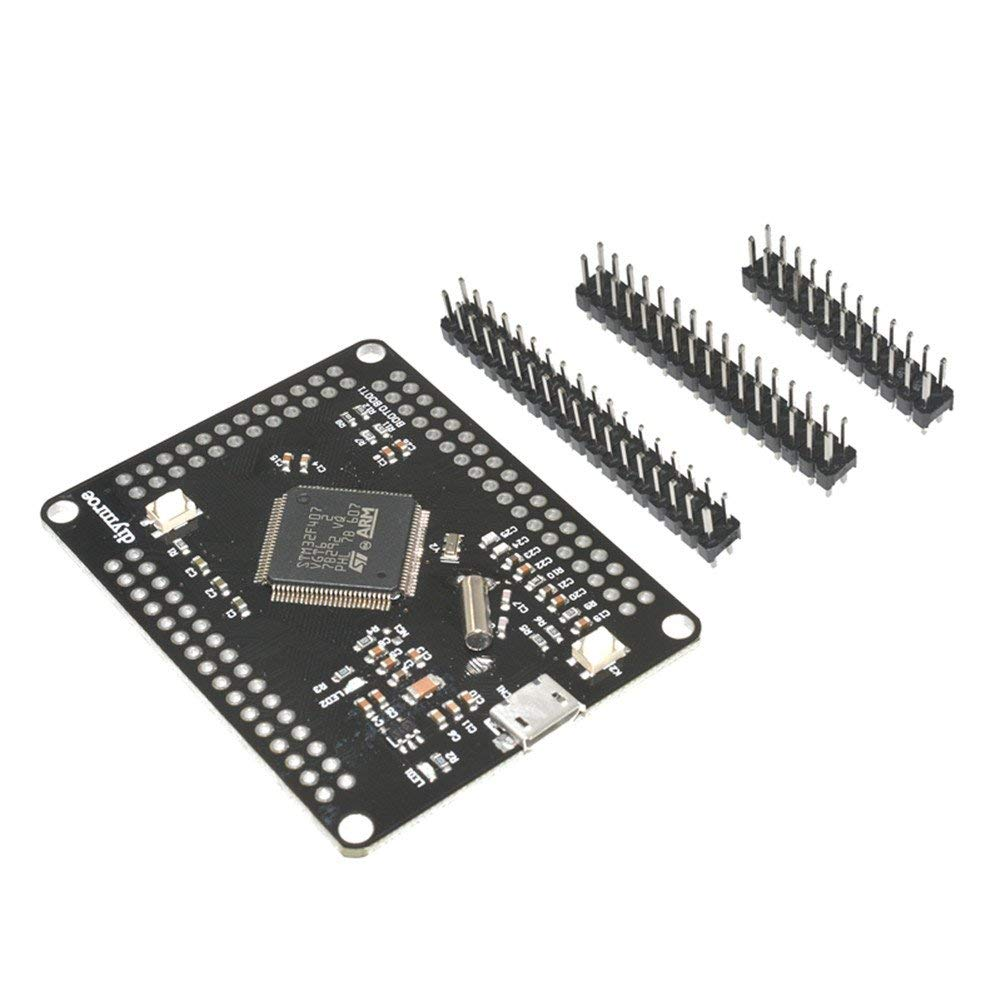
\includegraphics[width=1in]{../src/im/dev_board}
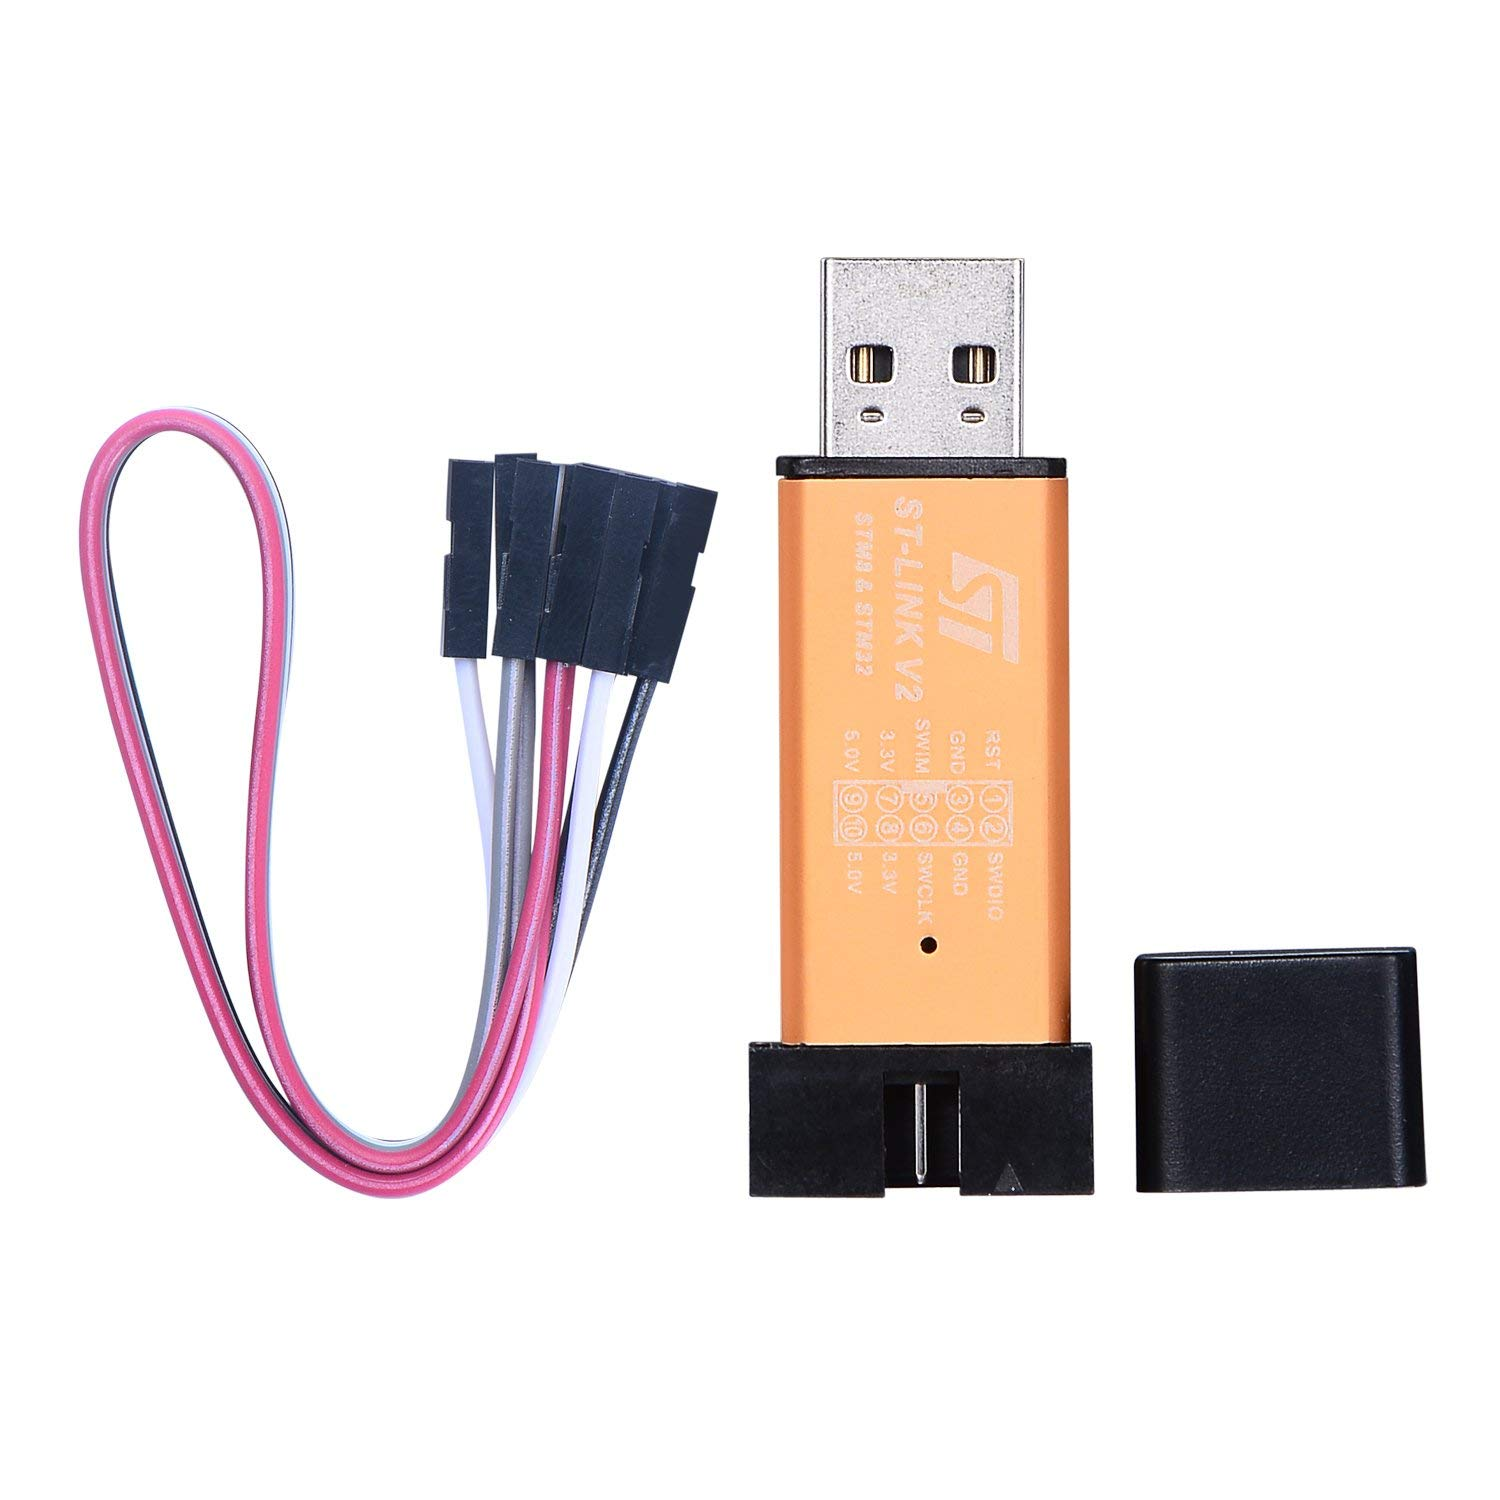
\includegraphics[width=1in]{../src/im/programmer}
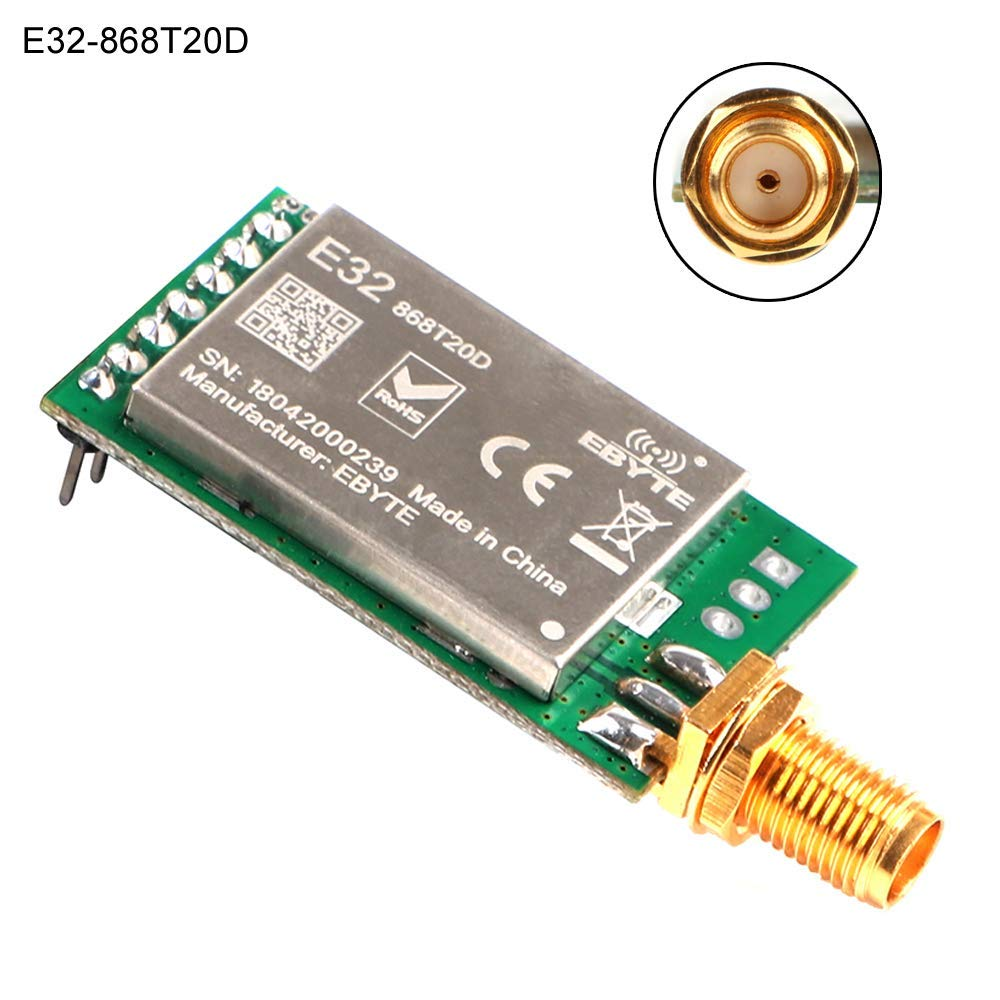
\includegraphics[width=1in]{../src/im/radio1}
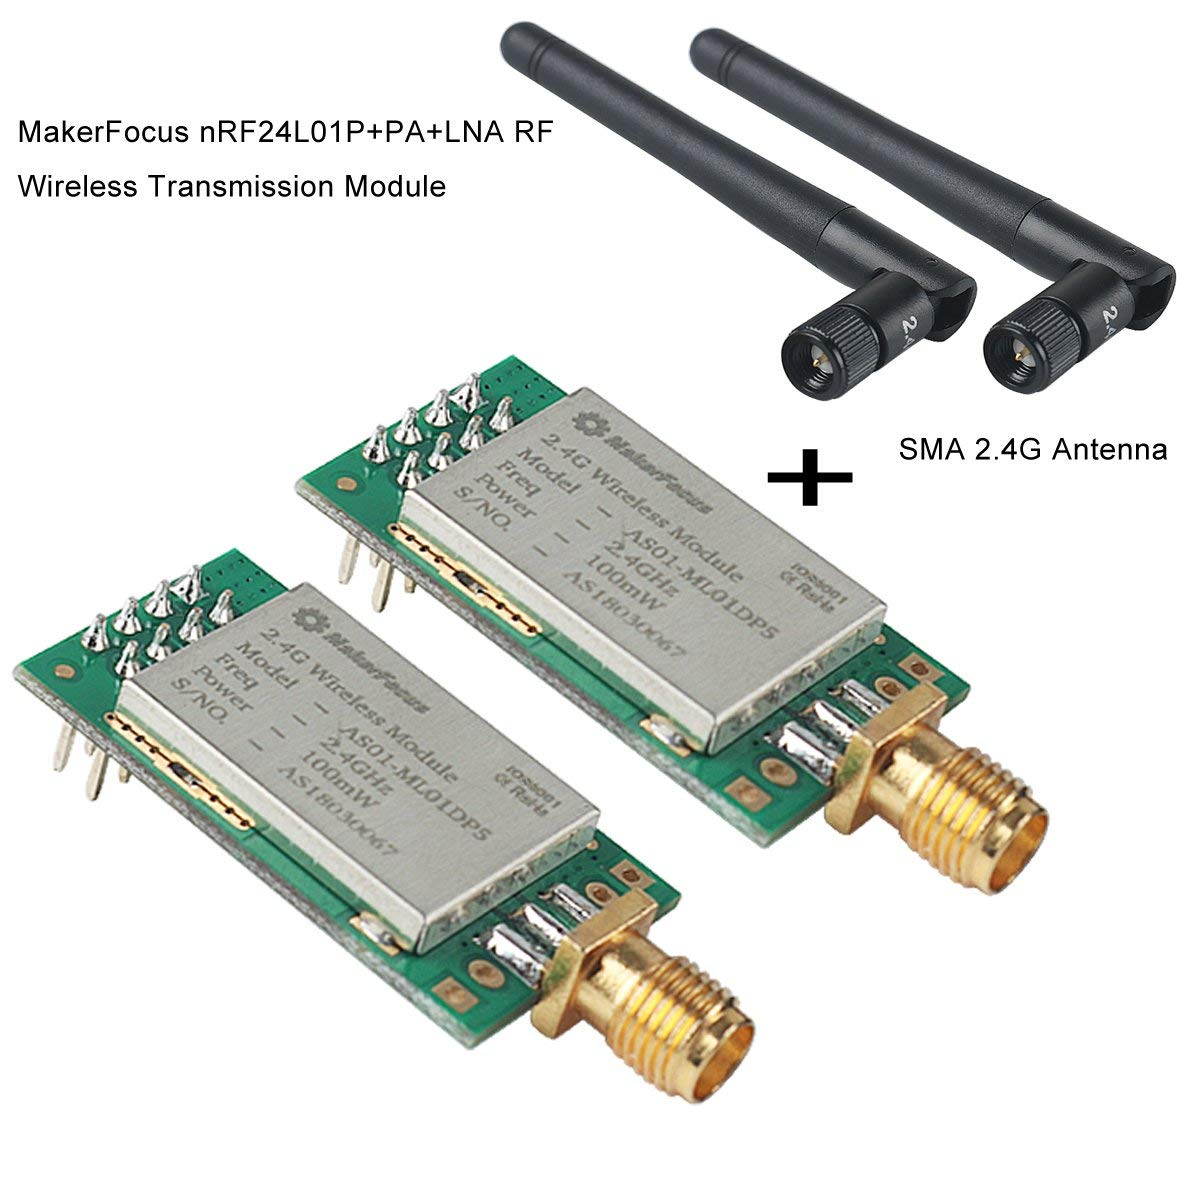
\includegraphics[width=1in]{../src/im/radio2}
\end{center}
\end{frame}

% ground station
\begin{frame}
\frametitle{Ground Station}
\begin{center}
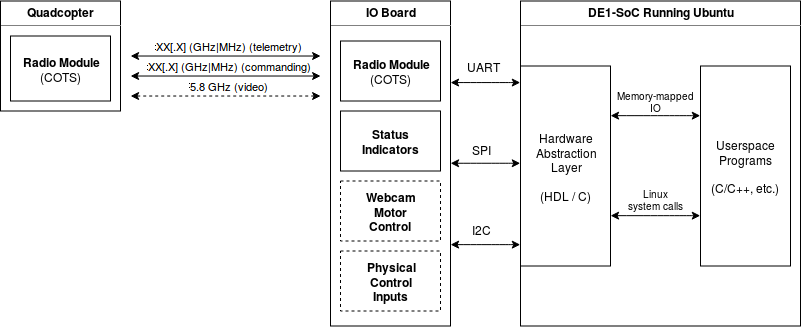
\includegraphics[width=\linewidth]{../src/im/ground_station}
\end{center}
\end{frame}

% display and controller
\begin{frame}
\frametitle{User Interface}
\begin{center}
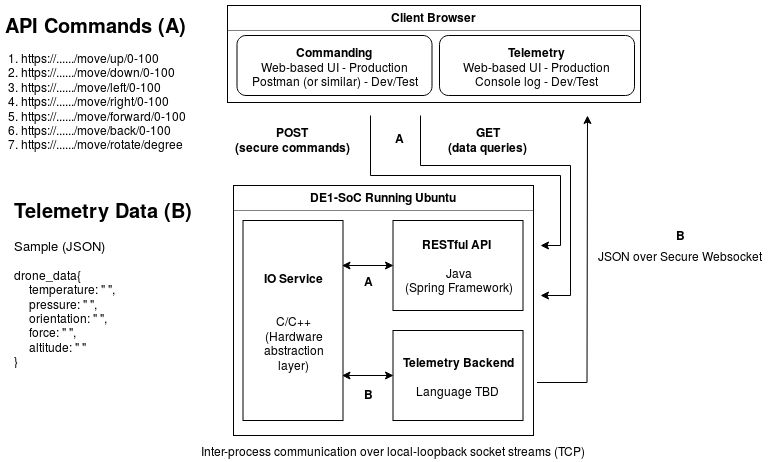
\includegraphics[height=225pt,width=\linewidth,keepaspectratio]{../src/im/display_controller}
\end{center}
\end{frame}

% total cost
\begin{frame}
\frametitle{Bill of Materials}
\begin{center}
\begin{tabular}{ c c c }
    cell 1 & cell 2 & cell 3 \\
    cell 4 & cell 5 & cell 6 \\
    cell 7 & cell 8 & cell 9
\end{tabular}
\end{center}
\end{frame}

\begin{frame}
\frametitle{Summary}
\large
We feel prepared to take on this challenge:
\begin{itemize}
    \item[\textbullet] Prior experience with systems' engineering (vehicle projects)
    \item[\textbullet] At least a dozen previous failures
    \item[\textbullet] Confident in this architecture
    \item[\textbullet] Have development tools and equipment on standby
\end{itemize}
\vspace{0.5in}
\begin{center}
Funding would greatly increase the quality of the final product!
\end{center}
\end{frame}

\end{document}
